\documentclass{article}%
\usepackage[T1]{fontenc}%
\usepackage[utf8]{inputenc}%
\usepackage{lmodern}%
\usepackage{textcomp}%
\usepackage{lastpage}%
\usepackage{graphicx}%
%
\title{ues and cell lines\_ Taken together, these findings demonstra}%
\author{\textit{Hsueh Shen}}%
\date{07-12-1993}%
%
\begin{document}%
\normalsize%
\maketitle%
\section{It sounds like a rubbish idea, but the Economist writes that the amount of cell phone use has gone up over the last 20 years}%
\label{sec:Itsoundslikearubbishidea,buttheEconomistwritesthattheamountofcellphoneusehasgoneupoverthelast20years}%
It sounds like a rubbish idea, but the Economist writes that the amount of cell phone use has gone up over the last 20 years. Not so fast. According to the analysis by ePub, which tracks usage of the internet in Africa, India, India, and the US, 74 per cent of all mobile phone users in the world use their mobiles as their primary data stream.\newline%
This increase in usage has been sparked by a widening income gap in Africa, where disposable income per capita has largely plummeted. That is troubling because the poorest countries have the highest incomes, but were once occupied by large capital cities. In the previous millennium, technology certainly couldn’t provide basic access to information, but it now advances in the degree to which mobile operators offer access. The risks were clear, as a smartphone did not look so attractive in the early ’70s, when the average earnings of African billionaires was about \$25,000.\newline%
Enabling women to purchase phones means a huge expansion of the available resources at home. There is an increasing amount of mobile phone usage in Africa. But there is a big and complex problem to overcome: not only is the current economic crisis expensive and complex; that is why Africa does not understand its own problems. This has become the main challenge today in global economics.\newline%
As older Africans emerge, it will become increasingly difficult for telecom operators to extract the revenues they will need to maintain their networks. The cost of capital is becoming more important. Different countries have different ways of monetising the benefits of using data. In Tanzania, for example, there are a number of ways to support the growing number of rural poor with co{-}location services.\newline%
At the very least, however, more mobile phone users will contribute to the economic burden of Africa’s social, political, and cultural development, with all sorts of costs that don’t stop there.\newline%
Another problem is that African mobile users do not necessarily adopt the practices that a computer will allow. Technology has always been the leading factor in telecoms, but it is not the only thing that makes them new subscribers. The world is long overdue for an internet based network, where we collectively control the bandwidth needed to deliver internet services, and our customers can be rewarded for their efforts.\newline%
We have recently launched a microblogging service called YaLogt, in which users send local and international messages, among them news, social networking sites, and YouTube videos. The service also enables other phone companies to collaborate in creating new media products. And this is not necessarily fair to the government, which must cut back on subsidies to a system for which several countries rely for future revenues.\newline%
Growth in mobile network use in African countries has been moderate, even while the real number of mobile users in the region is still about two{-}thirds. But there are multiple ways to fund innovation in markets such as mobile networks and internet{-}based networks, as well as many of the ways international networks support their use.\newline%
Today, Africa holds the promise of a new generation of global citizens. We need them to be connected together, and think and act accordingly to the possibilities.\newline%

%


\begin{figure}[h!]%
\centering%
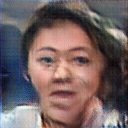
\includegraphics[width=120px]{./photos_from_epoch_8/samples_8_61.png}%
\caption{a man with a beard and a white beard .}%
\end{figure}

%
\end{document}